%----------------------------------------
% Preamble to set up the document
%----------------------------------------
\documentclass{article}

% set up packages (you shouldn't need to touch this)
\usepackage{graphicx}  % required to insert images
\usepackage{hyperref}  % for hyperlinks
\usepackage[svgnames]{xcolor}  % to change hyperlink colors
\colorlet{linkcolour}{DarkBlue}
\hypersetup{colorlinks=true, linkcolor=linkcolour, citecolor=linkcolour, urlcolor=linkcolour,}
\usepackage{subfigure}

% Margins
\topmargin=-0.45in
\evensidemargin=0in
\oddsidemargin=0in
\textwidth=6.5in
\textheight=9.0in
\headsep=0.25in

% use a sans serif font
\renewcommand{\familydefault}{\sfdefault}


%----------------------------------------
% Step 1: Edit the lecture title
%----------------------------------------
\title{
Lecture 2: Introduction to Counting \\  % Lecture title
Modeling Social Data, Spring 2019 \\   % Course title
Columbia University                    % School
}

%----------------------------------------
% Step 2: Edit your name and the date
%----------------------------------------
\author{Tanmay Chopra}                     % Scribe's name
\date{February 1, 2019}                % Lecture date



\begin{document}

\maketitle


%----------------------------------------
% Step 3:
% Rename uni.tex to match your uni,
% edit the filename accordingly below,
% and put your notes in this file
%----------------------------------------
%----------------------------------------
% Write your notes here
%----------------------------------------

\section{Introduction}
Counting is incredibly important. 80\% of Jake's research centers around knowing what to count and how to count it. Even estimating conditional probabilities is just counting!

\section{Example Application}
Finding the probability of supporting a particular candidate, given certain characteristics about the populace. For example:
$$\Pr(y|age) or \Pr(y|age,race) or \Pr(y|age,race,sex,party...) $$

To solve probabilities like these, we would simply count the number of people in that specific sub-group(people who meet the given characteristics) who support the candidate and divide by the total number of people in that subgroup. \textbf{It's just counting.}

\subsection{Question}
How many responses do we need to estimate p(y) with a 5\% margin of error?

\subsubsection{Aside}
What do we mean by 5\% margin of error?
\begin{itemize}
  \item Mean won't usually vary by more than 5\%
  \item Standard error will be 5\% that is, standard deviation of mean of sampling distribution will be 5\%
\end{itemize}

How would we do this practically? (illustrated through coin flips)\\
\textbf{Through simulations}. 


Just simulate flipping a coin 100 times and calculate mean value. Repeat experiment 100000 times and see distribution of means. 
We notice that uncertainty is highest when the probability of outcomes is evenly split (like here, when p(h) = p(t) = 0.5) because distinctions are clearer in case of skewed probabilities, which makes the mean distribution clearer.

\subsection{Relation between sample size and variance}
The all-important question of how many responses do we really need to get a specific margin of error can be better answered using the formula derived here.

\begin{equation}
  var( \frac{1}{n} \sum_{i=1}^{n}  x_i) = \frac{1}{n^2}var( \sum_{i=1}^{n}  x_i) 
\end{equation}
\begin{equation}
    = \frac{1}{n^2} \sum_{i=1}^{n} var(x_i) = \frac{1}{n^2}np(1-p)
\end{equation}
\begin{equation}
    = \frac{p(1-p)}{n}
\end{equation}

Now looking at standard deviation s,
 \begin{equation}
    s = \sqrt{\frac{p(1-p)}{n}}
\end{equation}
 \begin{equation}
    n = \frac{p(1-p)}{s^2}
\end{equation}
Where n is the number of samples. Hence,
\begin{equation}
    n \alpha \frac{1}{s^2}
\end{equation}



\subsection{The Challenge}
If we wanted to split our conditional probabilities even into just 100 age groups, 2 sexes, 5 races and 3 parties-a very basic split-we'd end up with 3000 separate groups and assuming we need a 100 data points to estimate probabilities for each group, we'd need 300,000 responses. Unfortunately, the usual survey only gets a few hundred or few thousand respondents. 
Hence, the brute force approach is not useful.

\subsubsection{Potential Solutions}
\begin{itemize}
  \item Use less groups, by binning small groups into bigger ones. This sacrifices granularity in data for precision
  \item Develop sophisticated methods that generalize well, like modeling
  \item Get more data!
\end{itemize}

\section{Diving into Research}
We then dove into a research paper on forecasting elections through non-representative sampling. The paper analyzed a poll taken through XBox, with 300,000+ responses.
Note: Working with larger samples is mathematically easier and sounds great, but can get computationally taxing and at very large scales, even impossible. So need to always analyze the trade-off between simpler analysis and more computation.

\section{Split-Apply-Combine}
An effective way to count data is the split-apply-combine method, where you simply arrange observations into groups,calculate their statistics individually and then collect those results.
\begin{figure}[ht]
  \begin{center}
    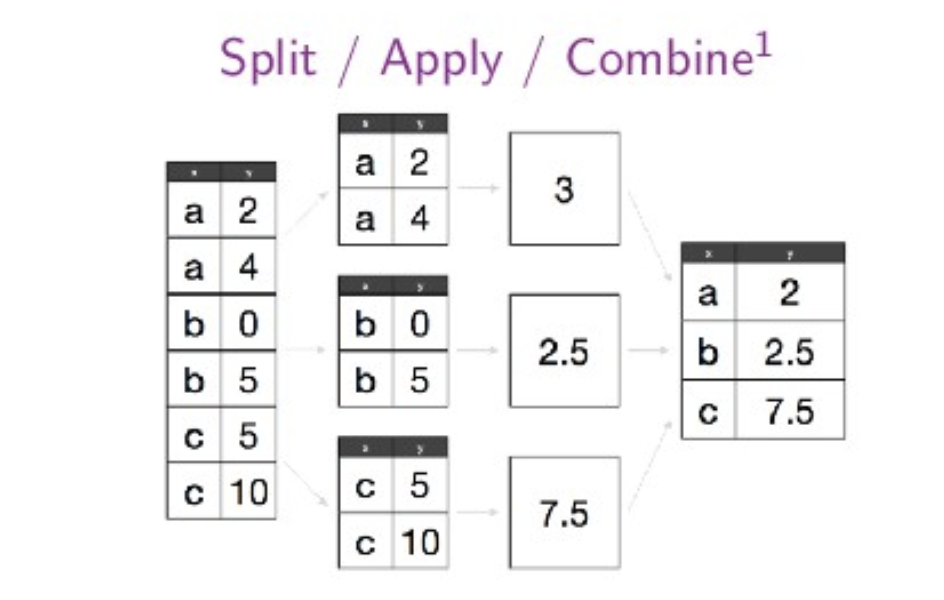
\includegraphics[width=0.5\textwidth]{figures/sac.png}
    \caption{
      Illustration of Split-Apply-Combine 
      From Lecture Slides, originally from The Split-Apply-Combine Strategy for Data Analysis by Hadley Wickam
      }
    \label{fig:example_figure}
  \end{center}
\end{figure}

\section{Methods of Computation}
We can often compute the same statistic in various different ways. Taking the example of computing averages, we saw how the computation space and time can vary greatly based on how we calculate the same statistic. 
Ways of computing the mean of each group:
\begin{enumerate}
  \item The Dumbest: Find all entries associated with a group and make a list of their values. Then get the average by summing up this list. Repeat for each group. \\
  Time: G x N where N is number of observations and G is number of groups\\
  Space: N (worst case is all observations are in one group so list is N elements long)
  \item Less Dumb: Create a list of each group. Run through observations, adding each observation to the list of the group to which it belongs.
  In the end, find the average for each list(group). \\
  Time: N\\
  Space: N
  \item Least Dumb: Keep a running average for each group that is, store two numbers per group - the sum of all observations and the count of observations of each group. \\
  Time: N \\
  Space: 2G (approximately equal to G)
\end{enumerate}


\section{Research Paper on Long Tails}
\subsection{Overview}
\paragraph{We then moved onto a research paper, "Anatomy of the Long Tail:
Ordinary People with Extraordinary Tastes" which explored whether the 'long tail' in inventory, or the massive list of rarely purchased goods arises from a few people having completely eclectic tastes, while others are completely mainstream or everyone having partially mainstream and partially eclectic tastes.}

\paragraph{The two datasets used for this experiment were the Netflix and MovieLens data sets, which varied in both granularity and sample size.\\
A set of graphs was computed, which helped us visualize the distribution of data.}

\subsection{Visualizing the Data}

\paragraph{We saw graphs for ratings vs number of ratings and a density vs rating graph to help us understand how the ratings were distributed. \\
We also saw a cumulative rating fraction graph that illustrated what fraction of the ratings were given to movies ranked in order of decreasing ratings. The steep decline in the slope beyond a certain point showed that most ratings were given to a select few movies, while most movies received very few ratings(the long tail).}

\paragraph{We then delved into the users and their preferences, studying the median rank of users' rated movies. This was defined as the eccentricity of the user and showed that most users were partially mainstream and partially eccentric in their tastes.}



\subsection{Additional Insights}
If size of data is larger than available memory, we can:
\begin{itemize}
  \item Use random sampling of the data, but this results in unreliable estimates for rare groups
  \item Randomly access the data from the disk- gives us 1000x storage but takes 1000x the time.
  \item Using streaming - read one observation at a time, storing only what you need.
\end{itemize}
Streaming algorithm is important!

\subsection{More Practical Examples}
We also touched on other examples, like Youtube videos, and explored how we could handle data of that scale and what could and could not be computed from that on a computer with 8Gb Ram 


\begin{figure}[h!]
  \begin{center}
\subfigure{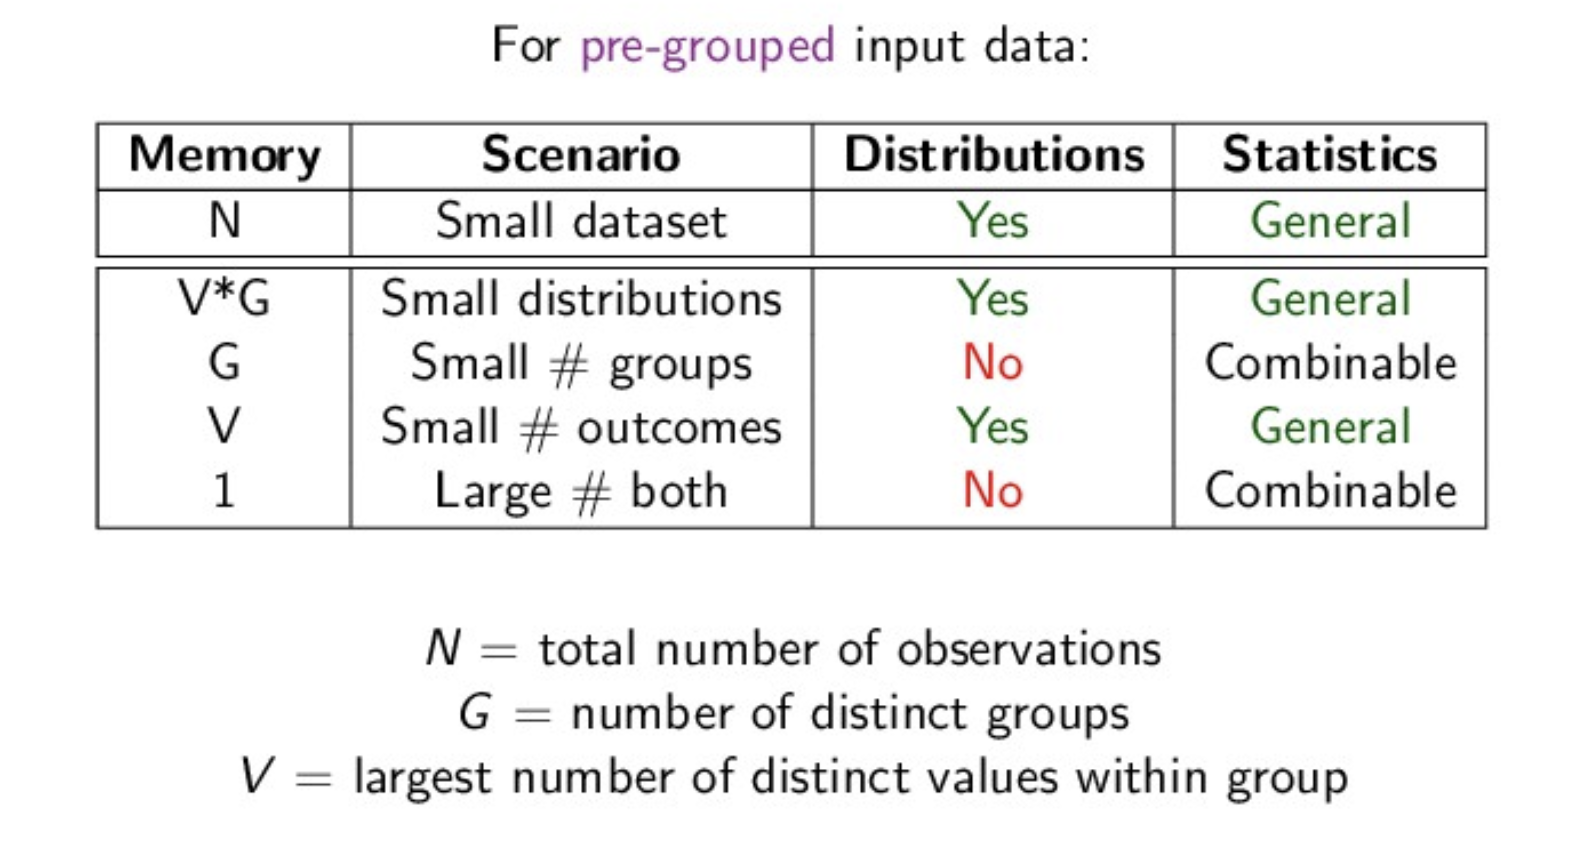
\includegraphics[width=8cm]{figures/pre_grouped_input.png}}
\subfigure{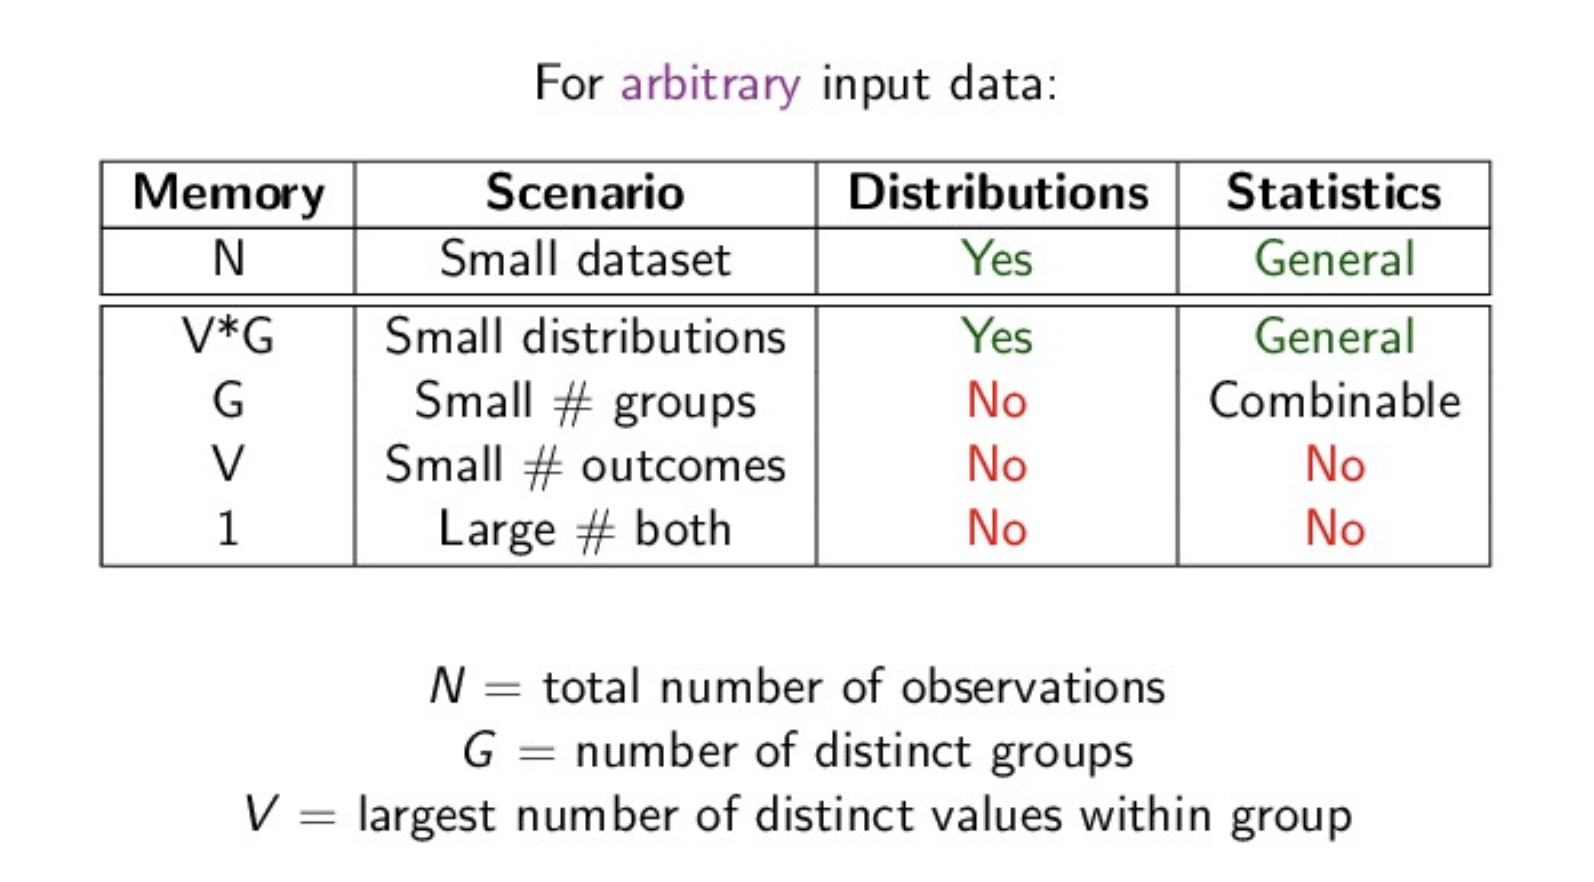
\includegraphics[width=8cm]{figures/arbitary_input.png}}
\caption{
      From Lecture Slides
      }
\end{center}
\end{figure}

     
     
\section{Introduction to Command Line}
We dove into the command line operations. Jake mentioned that it's worthwhile to know how to work with the command line largely because how quickly one can explore data through it, without having to load it anywhere or read into anything.
\begin{itemize}
  \item Moving around our disk - ls to list files in directory, pwd to find present working directory, moving into and out of directories with cd
  \item Distinguishing between the effects of using different types of quotes or no quotes
  \item Working with variables
  \item Working with pipes and understanding input/output streams as well as cat to display contents
  \item Running Scripts
\end{itemize}

\subsection{Playing Around with CitiBike Data}
We then conducted a basic exploratory data analysis of publicly available Citibike data to experiment with the operations we'd learnt.\\
We did some counting and pattern matching. We counted the number of distinct genders and looked up addresses similar to a particular pattern using grep among other things and even plotted a histogram on the command line interface!


\section{Important Formulae}
\begin{equation}
  var(\lambda x) = \lambda^2var(x)
\end{equation}
\begin{equation}
  var(x_1 + x_2) = var(x_1) + var(x_2)
\end{equation}

















\end{document}

%%% Local Variables:
%%% mode: latex
%%% TeX-master: t
%%% End:
